\documentclass[pdf,xcolor=dvipsnames,noparindent]{beamer}

\usetheme{Warsaw}
\usecolortheme{spruce}

% packages
\usepackage{listings}
% \usepackage{upquote}

% \lstset{numbers=left, numberstyle=\footnotesize, stepnumber=1,firstnumber=1,
%     numbersep=5pt,
%     stringstyle=5pt,
%     basicstyle=\footnotesize,
%     keepspaces=true, tabsize=4,
%     showstringspaces=false
%     % backgroundcolor=\color{SpringGreen}
% }

% preamble
\title{Introduction to Go - Part 1}
\author{Wojciech Gac}
\date{July 26, 2019}

% document proper
\begin{document}

\begin{frame}
	\titlepage
\end{frame}

% \begin{frame}{Outline}
% 	\pause
% 	\begin{itemize}
% 		\item The Problem
% 		      \pause
% 		\item Delve Debugger
% 		      \pause
% 		\item Container Preparation
% 		      \pause
% 		\item Debugging
% 		      \pause
% 		\item Further Reading
% 	\end{itemize}
% \end{frame}

% \begin{frame}
% 	\frametitle{The Problem}
% 	We'd like to be able to do the following:
% 	\pause
% 	\begin{itemize}
% 		\item Using a local instance of VSCode...
% 		      \pause
% 		\item ...and a dockerized instance of a Go application...
% 		      \pause
% 		\item ...connect to a running process \emph{inside} the container...
% 		      \pause
% 		\item ...interrupt execution with breakpoints and modify variables on the fly
% 	\end{itemize}
	  
% \end{frame}

\begin{frame}{Outline}
  \pause
  \begin{itemize}
  \item Origins of Go
    \pause
  \item Strong Points
    \pause
  \item Language Basics
    \pause
  \item Concurrency Patterns
    \pause
  \item Practical Use Cases
    \pause
  \end{itemize}
\end{frame}

\begin{frame}{Origins of Go}
  \pause
  \begin{itemize}
  \item Designed at Google in 2007
    \pause
  \item ... by Rob Pike, Ken Thompson and Robert Griesemer
    \pause
  \item ... two of whom (Pike \& Thompson) had spent decates at Bell Labs
    \pause
  \item ... building on a long history of concurrent languages
    \pause
  \item ... such as Occam, Erlang, Newsqueak, Concurrent ML, Alef and Limbo
  \end{itemize}
  
\end{frame}

\begin{frame}{Origins of Go}
  \pause
  \begin{itemize}
  \item Heavily influenced by Tony Hoare's CSP paper from 1978
    \begin{figure}
      \centering
      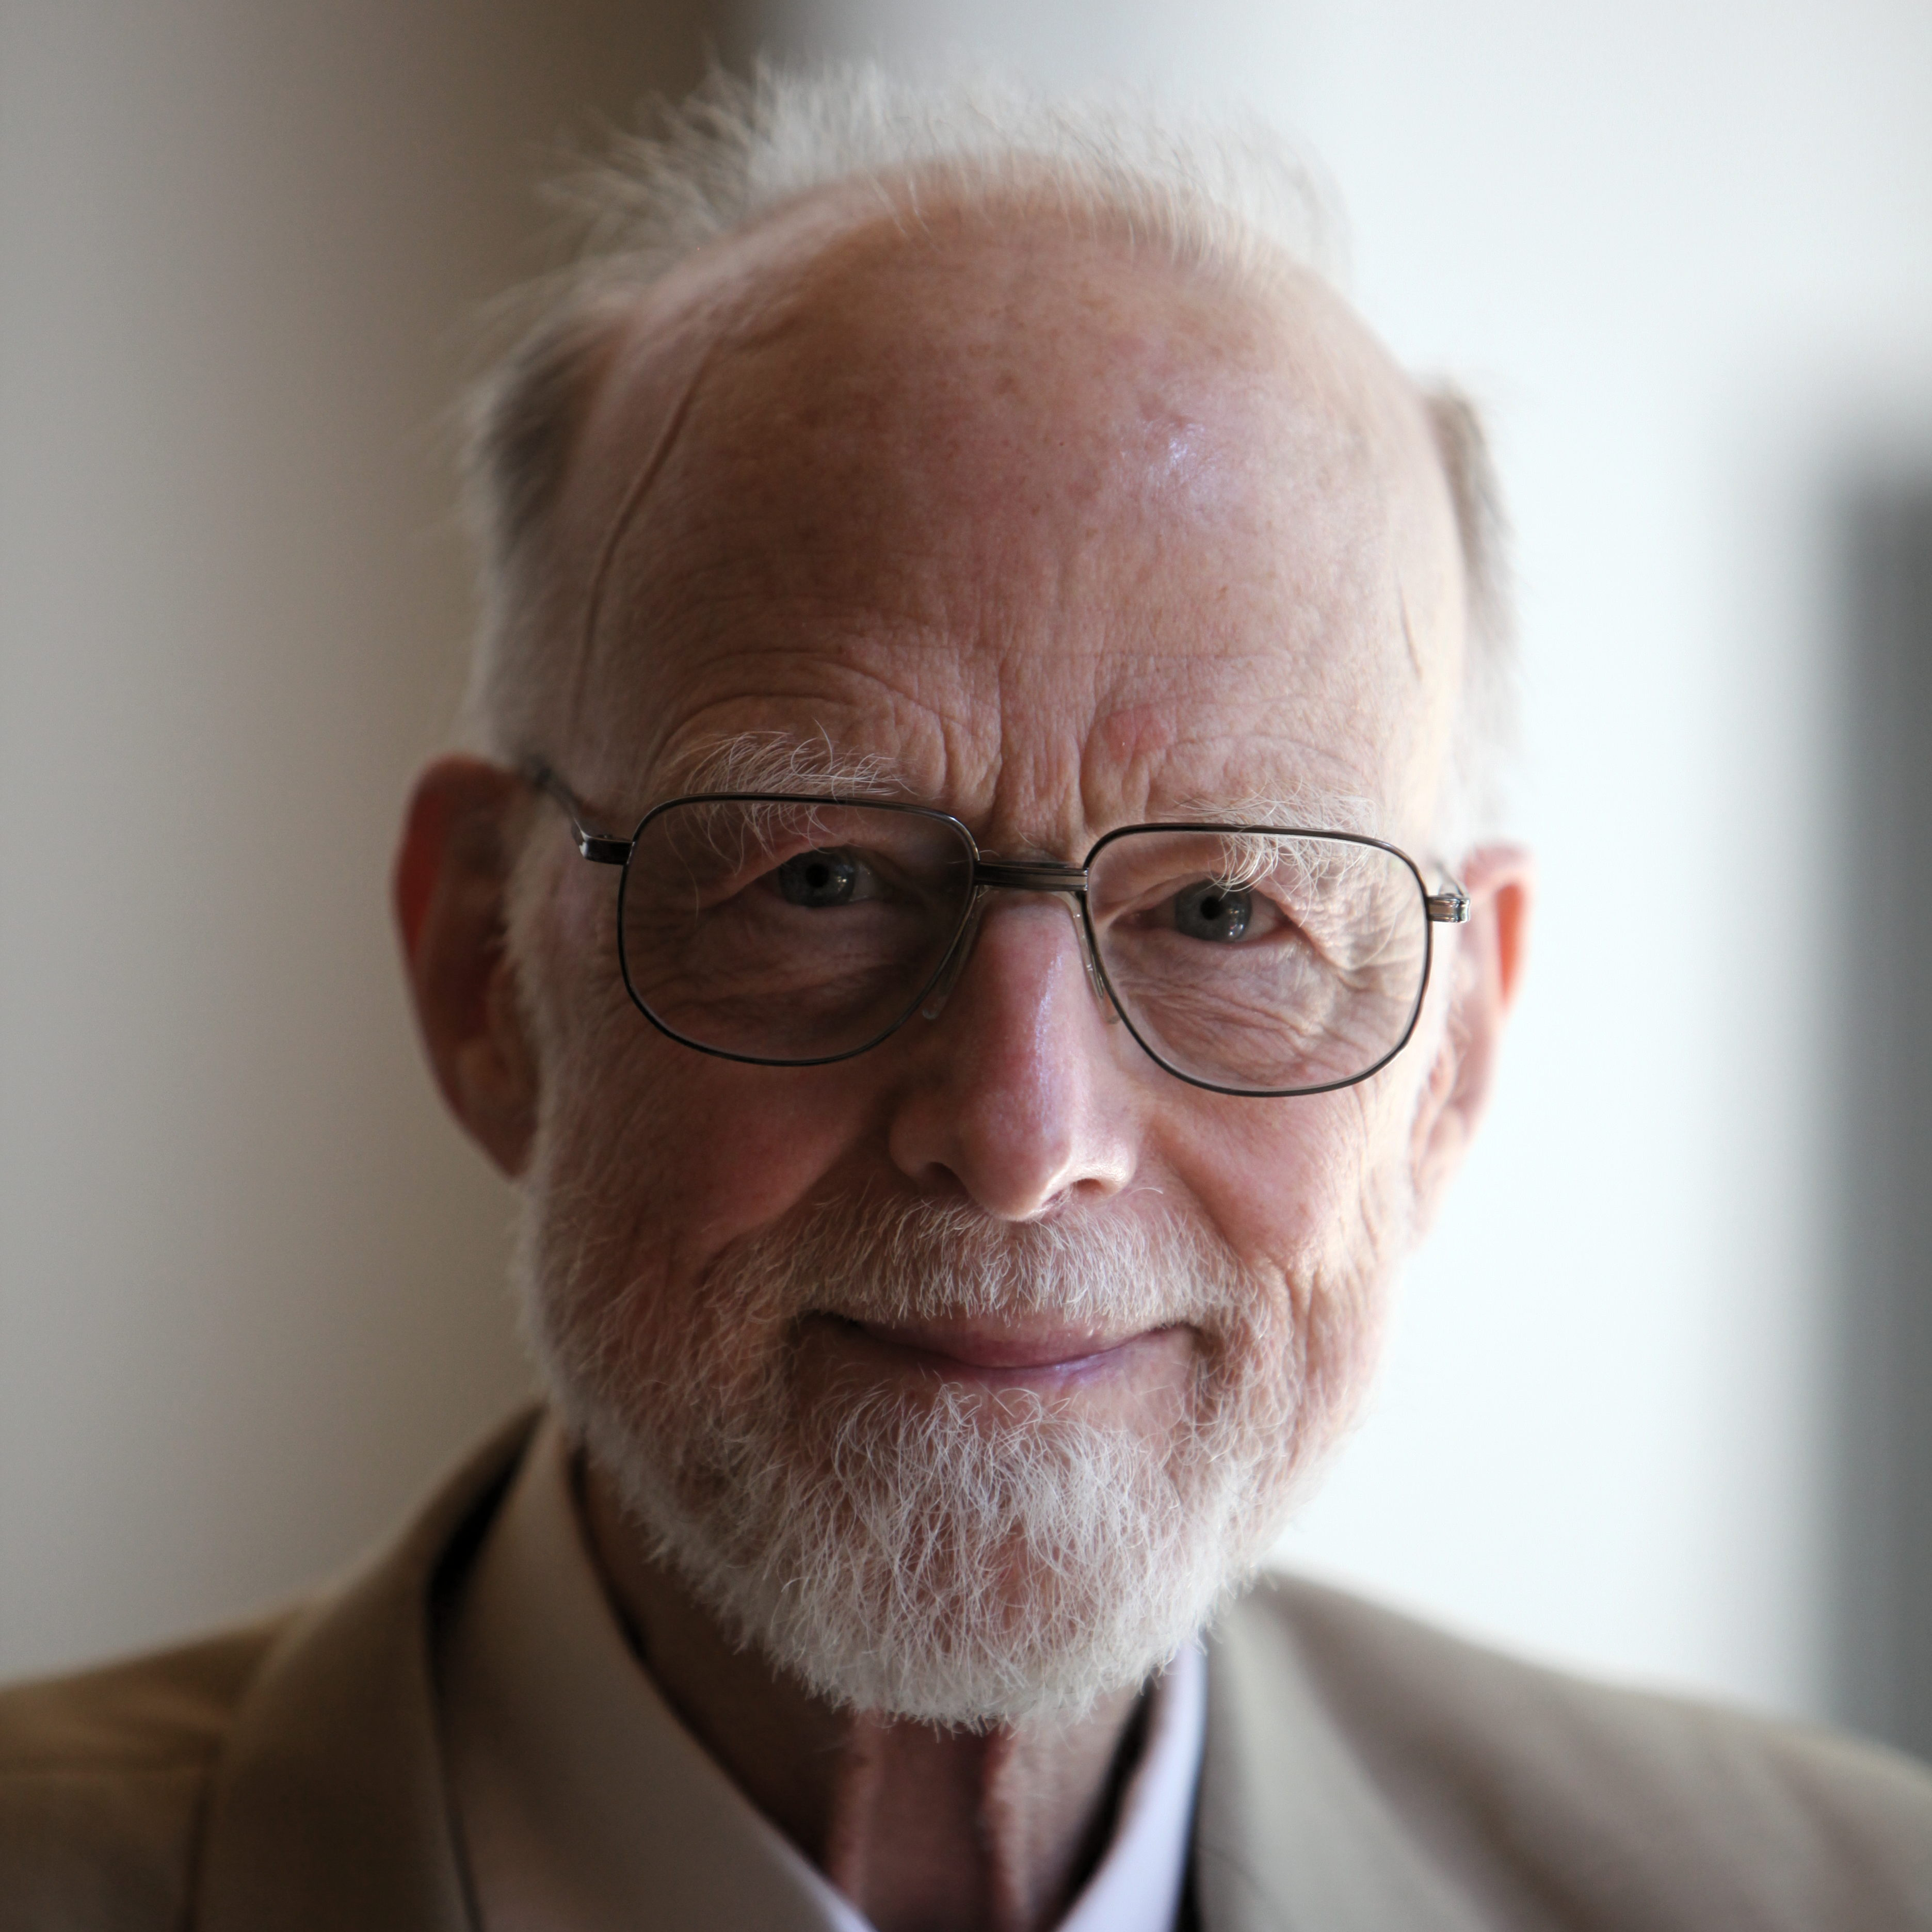
\includegraphics[scale = 0.02]{images/hoare.jpg}
    \end{figure}
    \pause
  \item ... in which input and output operations are programming primitives
    \pause
  \item ... helping structure parallel process communication
  \end{itemize}
  
\end{frame}


\end{document}